%%%%%%%%%%%%%%%%%%%%%%%%%%%%%%%%%%%%%%%%%%%%%%%%%%%%%%%%%%%%%%%%%%%%%%%%%%%%%%%
%                        WANDERIFY WHITEPAPER                                  %
%                    Travel-to-Earn on Polygon Network                         %
%%%%%%%%%%%%%%%%%%%%%%%%%%%%%%%%%%%%%%%%%%%%%%%%%%%%%%%%%%%%%%%%%%%%%%%%%%%%%%%

\documentclass[11pt,a4paper]{article}

%------------------------------------------------------------------------------
% PACKAGES
%------------------------------------------------------------------------------
\usepackage[utf8]{inputenc}
\usepackage[T1]{fontenc}
\usepackage{lmodern}
\usepackage[margin=1in]{geometry}
\usepackage{graphicx}
\usepackage{xcolor}
\usepackage{tikz}
\usetikzlibrary{shapes.geometric, arrows.meta, positioning, calc, shadows, decorations.pathreplacing}
\usepackage{tcolorbox}
\tcbuselibrary{skins,breakable}
\usepackage{fontawesome5}
\usepackage{hyperref}
\usepackage{fancyhdr}
\usepackage{titlesec}
\usepackage{enumitem}
\usepackage{booktabs}
\usepackage{tabularx}
\usepackage{amsmath}
\usepackage{amssymb}
\usepackage{multicol}
\usepackage{float}
\usepackage{caption}
\usepackage{subcaption}
\usepackage{lipsum}

%------------------------------------------------------------------------------
% COLOR DEFINITIONS - Polygon Inspired Palette
%------------------------------------------------------------------------------
\definecolor{polygonPurple}{HTML}{8247E5}
\definecolor{polygonDark}{HTML}{1A0A2E}
\definecolor{polygonLight}{HTML}{A67DFF}
\definecolor{polygonGradientStart}{HTML}{8247E5}
\definecolor{polygonGradientEnd}{HTML}{F2B8FF}
\definecolor{accentCyan}{HTML}{00D4FF}
\definecolor{accentGreen}{HTML}{00FF88}
\definecolor{accentOrange}{HTML}{FF9500}
\definecolor{textDark}{HTML}{1A1A2E}
\definecolor{textMuted}{HTML}{6B7280}
\definecolor{bgLight}{HTML}{F8F9FC}
\definecolor{cardBg}{HTML}{FFFFFF}

%------------------------------------------------------------------------------
% HYPERLINK SETUP
%------------------------------------------------------------------------------
\hypersetup{
    colorlinks=true,
    linkcolor=polygonPurple,
    urlcolor=accentCyan,
    citecolor=polygonPurple,
    pdftitle={Wanderify Whitepaper - Travel-to-Earn on Polygon},
    pdfauthor={Wanderify Team},
}

%------------------------------------------------------------------------------
% CUSTOM BOXES
%------------------------------------------------------------------------------
\newtcolorbox{highlightbox}[1][]{
    enhanced,
    colback=polygonPurple!5,
    colframe=polygonPurple,
    arc=4mm,
    boxrule=1.5pt,
    left=15pt,
    right=15pt,
    top=10pt,
    bottom=10pt,
    fonttitle=\bfseries\large,
    #1
}

\newtcolorbox{infobox}[1][]{
    enhanced,
    colback=accentCyan!5,
    colframe=accentCyan,
    arc=3mm,
    boxrule=1pt,
    left=12pt,
    right=12pt,
    #1
}

\newtcolorbox{warningbox}[1][]{
    enhanced,
    colback=accentOrange!10,
    colframe=accentOrange,
    arc=3mm,
    boxrule=1pt,
    left=12pt,
    right=12pt,
    #1
}

\newtcolorbox{successbox}[1][]{
    enhanced,
    colback=accentGreen!10,
    colframe=accentGreen,
    arc=3mm,
    boxrule=1pt,
    left=12pt,
    right=12pt,
    #1
}

%------------------------------------------------------------------------------
% SECTION STYLING
%------------------------------------------------------------------------------
\titleformat{\section}
    {\normalfont\LARGE\bfseries\color{polygonPurple}}
    {\thesection.}{0.5em}{}[\vspace{2pt}\titlerule]
    
\titleformat{\subsection}
    {\normalfont\Large\bfseries\color{polygonDark}}
    {\thesubsection}{0.5em}{}
    
\titleformat{\subsubsection}
    {\normalfont\large\bfseries\color{textDark}}
    {\thesubsubsection}{0.5em}{}

%------------------------------------------------------------------------------
% HEADER/FOOTER
%------------------------------------------------------------------------------
\pagestyle{fancy}
\fancyhf{}
\fancyhead[L]{\textcolor{polygonPurple}{\textbf{Wanderify}}}
\fancyhead[R]{\textcolor{textMuted}{Whitepaper v1.0}}
\fancyfoot[C]{\textcolor{textMuted}{\thepage}}
\renewcommand{\headrulewidth}{0.5pt}
\renewcommand{\headrule}{\hbox to\headwidth{\color{polygonPurple}\leaders\hrule height \headrulewidth\hfill}}

%------------------------------------------------------------------------------
% DOCUMENT START
%------------------------------------------------------------------------------
\begin{document}

%------------------------------------------------------------------------------
% TITLE PAGE
%------------------------------------------------------------------------------
\begin{titlepage}
    
\begin{tikzpicture}[remember picture,overlay]
        % Background gradient
        \fill[polygonDark] (current page.south west) rectangle (current page.north east);
        
        % Decorative circles
        \fill[polygonPurple,opacity=0.3] (current page.north east) ++(-4cm,-4cm) circle (8cm);
        \fill[polygonLight,opacity=0.2] (current page.south west) ++(3cm,3cm) circle (6cm);
        \fill[accentCyan,opacity=0.15] (current page.center) ++(5cm,-2cm) circle (4cm);
        
        % Polygon pattern (hexagons)
        \foreach \x in {0,2,...,20} {
            \foreach \y in {0,2,...,28} {
                \draw[polygonPurple!20,line width=0.3pt] 
                    (\x-10,\y-14) -- ++(60:0.5) -- ++(0:0.5) -- ++(-60:0.5) 
                    -- ++(-120:0.5) -- ++(180:0.5) -- cycle;
            }
        }
    \end{tikzpicture}
    
    \vspace*{3cm}
    
    \begin{center}
        % Logo placeholder
        
\begin{tikzpicture}
            \node[circle,fill=polygonPurple,minimum size=3cm,inner sep=0pt,
                  drop shadow={shadow xshift=0.1cm,shadow yshift=-0.1cm,opacity=0.3}] (logo) {};
            \node[white,font=\Huge\bfseries] at (logo) {\faPlane};
        \end{tikzpicture}
        
        \vspace{1cm}
        
        {\fontsize{48}{52}\selectfont\bfseries\textcolor{white}{WANDERIFY}}
        
        \vspace{0.5cm}
        
        {\Large\textcolor{polygonLight}{From On-Chain to On-Ground}}
        
        \vspace{1.5cm}
        
        
\begin{tikzpicture}
            \node[rounded corners=5pt,fill=polygonPurple,text=white,font=\large\bfseries,
                  inner sep=12pt] {WHITEPAPER v1.0};
        \end{tikzpicture}
        
        \vspace{0.8cm}
        
        {\large\textcolor{accentCyan}{Travel-to-Earn Protocol on Polygon Network}}
        
        \vspace{3cm}
        
        % Polygon logo representation
        \begin{tikzpicture}
            \node[text=white,font=\small] {Powered by};
        \end{tikzpicture}
        
        \vspace{0.3cm}
        
        
\begin{tikzpicture}
            \fill[polygonPurple] (0,0) -- (0.5,0.866) -- (1.5,0.866) -- (2,0) -- (1.5,-0.866) -- (0.5,-0.866) -- cycle;
            \node[white,font=\bfseries] at (1,0) {POLYGON};
        \end{tikzpicture}
        
        \vfill
        
        {\textcolor{textMuted}{January 2026}}
    \end{center}
\end{titlepage}

%------------------------------------------------------------------------------
% TABLE OF CONTENTS
%------------------------------------------------------------------------------
\newpage
\tableofcontents
\newpage

%------------------------------------------------------------------------------
% EXECUTIVE SUMMARY
%------------------------------------------------------------------------------
\section{Executive Summary}

\begin{highlightbox}[title={\faLightbulb\ The Vision}]
\textbf{Wanderify} transforms physical travel into verifiable, rewarding on-chain adventures. Built on Polygon, we connect \textit{on-chain intent} with \textit{on-ground proof}, creating the world's first sustainable travel-to-earn economy.
\end{highlightbox}

\vspace{0.5cm}

Wanderify introduces a revolutionary approach to travel incentivization:

\begin{itemize}[leftmargin=*]
    \item[\textcolor{polygonPurple}{\faBolt}] \textbf{Stake-First Economics}: Users commit funds before travel, proving genuine intent
    \item[\textcolor{accentCyan}{\faMapMarkerAlt}] \textbf{GPS + ZK Verification}: Polygon ID enables privacy-preserving location proofs
    \item[\textcolor{accentGreen}{\faRecycle}] \textbf{Circular Pool Economy}: Failed journeys fuel rewards for successful travelers
    \item[\textcolor{accentOrange}{\faImage}] \textbf{Journey NFTs}: ERC-721 collectibles prove completed adventures
\end{itemize}

\vspace{0.5cm}

\begin{center}
\begin{tikzpicture}[
    node distance=1.5cm,
    every node/.style={font=\small},
    box/.style={rectangle,rounded corners=8pt,draw=polygonPurple,line width=1.5pt,
                fill=white,minimum width=2.5cm,minimum height=1cm,align=center,
                drop shadow={shadow xshift=2pt,shadow yshift=-2pt,opacity=0.2}}
]
    \node[box] (stake) {\faCoins\ \textbf{STAKE}};
    \node[box,right=of stake] (travel) {\faPlane\ \textbf{TRAVEL}};
    \node[box,right=of travel] (prove) {\faCheckCircle\ \textbf{PROVE}};
    \node[box,right=of prove] (earn) {\faTrophy\ \textbf{EARN}};
    
    \draw[-{Stealth[length=3mm]},line width=2pt,polygonPurple] (stake) -- (travel);
    \draw[-{Stealth[length=3mm]},line width=2pt,polygonPurple] (travel) -- (prove);
    \draw[-{Stealth[length=3mm]},line width=2pt,polygonPurple] (prove) -- (earn);
\end{tikzpicture}
\end{center}

%------------------------------------------------------------------------------
% THE PITCH
%------------------------------------------------------------------------------
\section{The Pitch}

\subsection{One-Liner}

\begin{center}

\begin{tikzpicture}
    \node[rounded corners=10pt,fill=polygonDark,text=white,font=\Large,
          inner sep=20pt,text width=14cm,align=center] {
        \textit{``Stake your commitment. Travel the world. Prove you arrived. Earn your reward.''}
    };
\end{tikzpicture}
\end{center}

\subsection{The Wanderify Promise}

\begin{multicols}{2}

\textbf{For Travelers:}
\begin{itemize}[leftmargin=*]
    \item Turn every journey into a financial opportunity
    \item Gasless transactions via meta-transactions
    \item Collect unique Journey NFTs
    \item Compete on global leaderboards
\end{itemize}

\columnbreak

\textbf{For the Ecosystem:}
\begin{itemize}[leftmargin=*]
    \item Self-sustaining token economy
    \item Real yield from DeFi integration
    \item Growing pool rewards over time
    \item Anti-fraud ZK verification
\end{itemize}

\end{multicols}

\subsection{Why Now?}

\begin{table}[H]
\centering
\begin{tabularx}{\textwidth}{>{\bfseries}l X}
\toprule
\textcolor{polygonPurple}{Market Trend} & \textcolor{textDark}{Wanderify Response} \\
\midrule
Web3 gaming saturation & First mover in \textit{real-world} earn mechanics \\
Travel industry recovery & \$9.5T global travel market ready for innovation \\
NFT utility demand & NFTs that prove real experiences, not just art \\
Polygon ecosystem growth & Native integration with Polygon ID, Lens, Aave \\
\bottomrule
\end{tabularx}
\end{table}

%------------------------------------------------------------------------------
% THE PROBLEM
%------------------------------------------------------------------------------
\section{The Problem}

\begin{warningbox}
\textbf{\faExclamationTriangle\ The Current State of Travel + Web3}

Despite billions traveling annually, there is \textbf{no protocol} that verifiably connects on-chain intent with on-ground movement. Travel remains an unmonetized, unverifiable action in the Web3 space.
\end{warningbox}

\subsection{Problem Breakdown}

\begin{figure}[H]
\centering
\begin{tikzpicture}[
    problem/.style={rectangle,rounded corners=8pt,draw=accentOrange,line width=1.5pt,
                    fill=accentOrange!10,minimum width=4cm,minimum height=2cm,
                    align=center,font=\small},
    arrow/.style={-{Stealth},line width=1pt,textMuted}
]
    % Problem 1
    \node[problem] (p1) at (0,0) {
        \textcolor{accentOrange}{\faEyeSlash}\\[5pt]
        \textbf{No Verifiable Travel}\\
        Photos \& posts are\\
        easily faked
    };
    
    % Problem 2
    \node[problem] (p2) at (5.5,0) {
        \textcolor{accentOrange}{\faChartLine}\\[5pt]
        \textbf{Weak Tokenomics}\\
        Existing apps rely on\\
        inflationary rewards
    };
    
    % Problem 3
    \node[problem] (p3) at (11,0) {
        \textcolor{accentOrange}{\faUnlink}\\[5pt]
        \textbf{Missing Link}\\
        No bridge between\\
        intent \& proof
    };
\end{tikzpicture}
\caption{The Three Core Problems in Travel-to-Earn}
\end{figure}

\subsection{Detailed Analysis}

\begin{enumerate}[label=\textcolor{polygonPurple}{\arabic*.},leftmargin=*]
    \item \textbf{Verification Gap}
    \begin{itemize}
        \item GPS can be spoofed with simple apps
        \item Photo metadata is easily manipulated
        \item IP-based checks are bypassed with VPNs
        \item No privacy-preserving verification exists
    \end{itemize}
    
    \item \textbf{Economic Sustainability}
    \begin{itemize}
        \item Current ``earn'' apps print tokens endlessly
        \item No skin-in-the-game from users
        \item Rewards come from token inflation, not real value
        \item Death spiral when token price drops
    \end{itemize}
    
    \item \textbf{User Experience}
    \begin{itemize}
        \item Complex wallet interactions
        \item High gas fees for microtransactions
        \item No engaging visual experience
        \item Fragmented social features
    \end{itemize}
\end{enumerate}

%------------------------------------------------------------------------------
% THE SOLUTION
%------------------------------------------------------------------------------
\section{The Solution}

\begin{successbox}
\textbf{\faRocket\ Wanderify's Answer}

A \textbf{stake-first, circular-pool economy} with \textbf{ZK-verified location proofs} on Polygon, delivering gasless UX and sustainable rewards.
\end{successbox}

\subsection{Solution Architecture Overview}

\begin{figure}[H]
\centering
\begin{tikzpicture}[
    scale=0.9,
    layer/.style={rectangle,rounded corners=10pt,minimum width=14cm,minimum height=2cm,
                  align=center,font=\bfseries},
    component/.style={rectangle,rounded corners=5pt,fill=white,draw=#1,line width=1pt,
                      minimum width=2.8cm,minimum height=1cm,align=center,font=\small}
]
    % Layer 1 - User Layer
    \node[layer,fill=accentCyan!20,draw=accentCyan,line width=2pt] (l1) at (0,6) {};
    \node[above=0.1cm of l1.north,font=\bfseries\color{accentCyan}] {USER LAYER};
    
    \node[component=accentCyan] at (-4,6) {\faGlobe\ Web App};
    \node[component=accentCyan] at (0,6) {\faMobile\ Mobile};
    \node[component=accentCyan] at (4,6) {\faWallet\ Wallet};
    
    % Layer 2 - Application Layer
    \node[layer,fill=polygonPurple!20,draw=polygonPurple,line width=2pt] (l2) at (0,3.5) {};
    \node[above=0.1cm of l2.north,font=\bfseries\color{polygonPurple}] {APPLICATION LAYER};
    
    \node[component=polygonPurple] at (-4.5,3.5) {\faMapMarkedAlt\ Navigation};
    \node[component=polygonPurple] at (-1.5,3.5) {\faCoins\ Staking};
    \node[component=polygonPurple] at (1.5,3.5) {\faCheckDouble\ Verification};
    \node[component=polygonPurple] at (4.5,3.5) {\faImage\ NFT Minting};
    
    % Layer 3 - Protocol Layer
    \node[layer,fill=accentGreen!20,draw=accentGreen,line width=2pt] (l3) at (0,1) {};
    \node[above=0.1cm of l3.north,font=\bfseries\color{accentGreen}] {PROTOCOL LAYER};
    
    \node[component=accentGreen] at (-4,1) {\faFingerprint\ Polygon ID};
    \node[component=accentGreen] at (0,1) {\faUsers\ Lens Protocol};
    \node[component=accentGreen] at (4,1) {\faChartPie\ Aave Yield};
    
    % Layer 4 - Blockchain Layer
    \node[layer,fill=polygonDark,draw=polygonDark,line width=2pt] (l4) at (0,-1.5) {};
    \node[above=0.1cm of l4.north,font=\bfseries\color{white}] {BLOCKCHAIN LAYER};
    
    \node[component=polygonPurple,fill=polygonDark,text=white] at (-3,-1.5) {\faFileContract\ Smart Contracts};
    \node[component=polygonPurple,fill=polygonDark,text=white] at (3,-1.5) {\faCubes\ Polygon PoS};
    
    % Arrows
    \draw[-{Stealth},line width=1.5pt,polygonPurple!60] (l1.south) -- (l2.north);
    \draw[-{Stealth},line width=1.5pt,polygonPurple!60] (l2.south) -- (l3.north);
    \draw[-{Stealth},line width=1.5pt,polygonPurple!60] (l3.south) -- (l4.north);
\end{tikzpicture}
\caption{Wanderify Four-Layer Architecture}
\end{figure}

\subsection{Core Mechanisms}

\subsubsection{1. Stake-First Economics}

\begin{infobox}
Users must stake tokens \textbf{before} their journey, creating genuine commitment and funding the reward pool.
\end{infobox}

\begin{table}[H]
\centering
\begin{tabularx}{\textwidth}{l X r}
\toprule
\textbf{Parameter} & \textbf{Description} & \textbf{Value} \\
\midrule
Minimum Stake Duration & Lock period before travel date & 15 days \\
Platform Fee & Fee sent to treasury & 4\% \\
Pool Deposit & Amount added to destination pool & 96\% \\
Claim Window & Time to verify after arrival & 24 hours \\
\bottomrule
\end{tabularx}
\caption{Staking Parameters}
\end{table}

\subsubsection{2. Circular Pool Economy}

\begin{figure}[H]
\centering
\begin{tikzpicture}[
    node distance=2cm,
    box/.style={rectangle,rounded corners=8pt,draw=#1,line width=1.5pt,fill=#1!10,
                minimum width=3cm,minimum height=1.5cm,align=center,font=\small\bfseries}
]
    % Central Pool
    \node[box=polygonPurple,minimum width=4cm,minimum height=2cm] (pool) at (0,0) {
        \faDatabase\\[3pt]
        DESTINATION\\POOL
    };
    
    % User Stake
    \node[box=accentCyan] (stake) at (-5,2) {\faUser\ USER\\STAKE};
    
    % Treasury
    \node[box=accentOrange] (treasury) at (-5,-2) {\faUniversity\ TREASURY\\(4\%)};
    
    % Success
    \node[box=accentGreen] (success) at (5,2) {\faCheckCircle\ SUCCESS\\Stake + Reward};
    
    % Failure
    \node[box=red!70] (failure) at (5,-2) {\faTimesCircle\ FAILURE\\Stays in Pool};
    
    % Arrows
    \draw[-{Stealth},line width=2pt,accentCyan] (stake) -- node[above,sloped,font=\scriptsize] {96\%} (pool);
    \draw[-{Stealth},line width=2pt,accentOrange] (stake) -- node[below,sloped,font=\scriptsize] {4\%} (treasury);
    \draw[-{Stealth},line width=2pt,accentGreen] (pool) -- node[above,sloped,font=\scriptsize] {Payout} (success);
    \draw[-{Stealth},line width=2pt,red!70,dashed] (pool) -- node[below,sloped,font=\scriptsize] {Locked} (failure);
    
    % Recycle arrow
    \draw[-{Stealth},line width=1.5pt,red!70] (failure.south) to[out=-90,in=-90,looseness=1.5] 
        node[below,font=\scriptsize] {Funds Future Winners} (pool.south);
\end{tikzpicture}
\caption{Circular Pool Economy Flow}
\end{figure}

\subsubsection{3. Reward Formula}

The emission calculation ensures sustainable rewards:

\begin{equation}
\boxed{
E = \min\left( R_{base} \times \left(1 + \frac{\beta \times PV}{100}\right), \quad Pool \times 10\% \right)
}
\end{equation}

\vspace{0.3cm}

\begin{table}[H]
\centering
\begin{tabularx}{\textwidth}{l X l}
\toprule
\textbf{Variable} & \textbf{Description} & \textbf{Default} \\
\midrule
$R_{base}$ & Base reward per check-in & 0.002 MATIC \\
$\beta$ & Place value multiplier & 50 (0.5 scaled) \\
$PV$ & Destination difficulty (0-100) & Varies \\
$Pool$ & Current pool balance & Dynamic \\
\bottomrule
\end{tabularx}
\end{table}

\textbf{Total Payout:}
\begin{equation}
\text{Payout} = \text{AmountInPool} + E
\end{equation}

\subsection{Polygon-Native Integrations}

\begin{figure}[H]
\centering
\begin{tikzpicture}[
    integration/.style={rectangle,rounded corners=10pt,draw=polygonPurple,line width=2pt,
                        fill=white,minimum width=3.5cm,minimum height=2.5cm,align=center},
    desc/.style={font=\scriptsize,text width=3cm,align=center}
]
    % Polygon ID
    \node[integration] (pid) at (0,0) {
        \textcolor{polygonPurple}{\faFingerprint}\\[5pt]
        \textbf{Polygon ID}
    };
    \node[desc,below=0.5cm of pid] {ZK-based identity\\Location credentials\\Privacy-preserving};
    
    % Lens Protocol
    \node[integration] (lens) at (5,0) {
        \textcolor{accentGreen}{\faLeaf}\\[5pt]
        \textbf{Lens Protocol}
    };
    \node[desc,below=0.5cm of lens] {Social travel feed\\Journey sharing\\Streak rewards};
    
    % Aave
    \node[integration] (aave) at (10,0) {
        \textcolor{accentCyan}{\faChartLine}\\[5pt]
        \textbf{Aave}
    };
    \node[desc,below=0.5cm of aave] {Yield on idle pools\\Real sustainable APY\\Auto-compound};
    
    % Biconomy
    \node[integration] (bico) at (2.5,-4) {
        \textcolor{accentOrange}{\faGasPump}\\[5pt]
        \textbf{Biconomy}
    };
    \node[desc,below=0.5cm of bico] {Gasless transactions\\Meta-transactions\\Seamless UX};
    
    % Chainlink
    \node[integration] (link) at (7.5,-4) {
        \textcolor{blue!70}{\faLink}\\[5pt]
        \textbf{Chainlink}
    };
    \node[desc,below=0.5cm of link] {Decentralized oracles\\Automated keepers\\Price feeds};
\end{tikzpicture}
\caption{Polygon Ecosystem Integrations}
\end{figure}

%------------------------------------------------------------------------------
% TECHNICAL ARCHITECTURE
%------------------------------------------------------------------------------
\section{Technical Architecture}

\subsection{Smart Contract Design}

\begin{figure}[H]
\centering
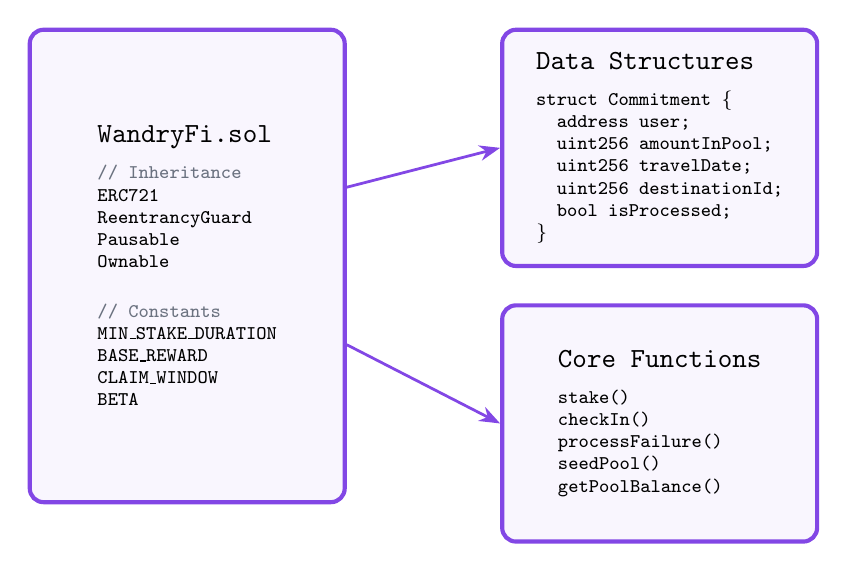
\begin{tikzpicture}[
    contract/.style={rectangle,rounded corners=5pt,draw=polygonPurple,line width=1.5pt,
                     fill=polygonPurple!5,minimum width=4cm,align=left,font=\ttfamily\scriptsize},
    inherit/.style={-{Triangle},line width=1pt,dashed,textMuted}
]
    % Main Contract
    \node[contract,minimum height=6cm] (main) at (0,0) {
        \textbf{\normalsize WandryFi.sol}\\[5pt]
        \textcolor{textMuted}{// Inheritance}\\
        ERC721\\
        ReentrancyGuard\\
        Pausable\\
        Ownable\\[10pt]
        \textcolor{textMuted}{// Constants}\\
        MIN\_STAKE\_DURATION\\
        BASE\_REWARD\\
        CLAIM\_WINDOW\\
        BETA
    };
    
    % Structs
    \node[contract,minimum height=3cm] (structs) at (6,1.5) {
        \textbf{\normalsize Data Structures}\\[5pt]
        struct Commitment \{\\
        \quad address user;\\
        \quad uint256 amountInPool;\\
        \quad uint256 travelDate;\\
        \quad uint256 destinationId;\\
        \quad bool isProcessed;\\
        \}
    };
    
    % Functions
    \node[contract,minimum height=3cm] (funcs) at (6,-2) {
        \textbf{\normalsize Core Functions}\\[5pt]
        stake()\\
        checkIn()\\
        processFailure()\\
        seedPool()\\
        getPoolBalance()
    };
    
    % Arrows
    \draw[-{Stealth},line width=1pt,polygonPurple] (main.east) ++(0,1) -- (structs.west);
    \draw[-{Stealth},line width=1pt,polygonPurple] (main.east) ++(0,-1) -- (funcs.west);
\end{tikzpicture}
\caption{Smart Contract Structure}
\end{figure}

\subsection{Verification Pipeline}

\begin{figure}[H]
\centering
\begin{tikzpicture}[
    node distance=0.8cm,
    step/.style={rectangle,rounded corners=5pt,draw=polygonPurple,line width=1pt,
                 fill=white,minimum width=4cm,minimum height=1cm,align=center,font=\small},
    arrow/.style={-{Stealth},line width=1.5pt,polygonPurple}
]
    % Steps
    \node[step] (s1) {\faLocationArrow\ GPS Coordinates Captured};
    \node[step,below=of s1] (s2) {\faKey\ API Key Validation};
    \node[step,below=of s2] (s3) {\faFingerprint\ Polygon ID Verification};
    \node[step,below=of s3] (s4) {\faCalculator\ Haversine Distance Check};
    \node[step,below=of s4] (s5) {\faPen\ Generate ECDSA Signature};
    \node[step,below=of s5,fill=accentGreen!20,draw=accentGreen] (s6) {\faCheckDouble\ On-Chain Verification};
    
    % Arrows
    \draw[arrow] (s1) -- (s2);
    \draw[arrow] (s2) -- (s3);
    \draw[arrow] (s3) -- (s4);
    \draw[arrow] (s4) -- (s5);
    \draw[arrow] (s5) -- (s6);
    
    % Side notes
    \node[right=1cm of s3,font=\scriptsize,text=textMuted,text width=4cm] {
        ZK-proof of location\\
        No raw GPS exposed
    };
    
    \node[right=1cm of s4,font=\scriptsize,text=textMuted,text width=4cm] {
        Must be $\leq$ 50m\\
        from destination
    };
\end{tikzpicture}
\caption{Location Verification Pipeline}
\end{figure}

\subsection{System Architecture Diagram}

\begin{figure}[H]
\centering
\begin{tikzpicture}[
    scale=0.85,
    component/.style={rectangle,rounded corners=8pt,draw=#1,line width=1.5pt,
                      fill=#1!10,minimum width=2.5cm,minimum height=1.2cm,
                      align=center,font=\small},
    db/.style={cylinder,draw=#1,line width=1.5pt,fill=#1!10,
               shape border rotate=90,aspect=0.3,minimum width=1.5cm,
               minimum height=1.5cm,font=\small},
    arrow/.style={-{Stealth},line width=1pt,textMuted}
]
    % Frontend
    \node[component=accentCyan] (frontend) at (0,4) {\faReact\ Next.js\\Frontend};
    
    % Backend
    \node[component=polygonPurple] (backend) at (5,4) {\faServer\ Node.js\\Backend};
    
    % Blockchain
    \node[component=polygonDark,text=white] (chain) at (10,4) {\faCubes\ Polygon\\Contracts};
    
    % IPFS
    \node[db=accentOrange] (ipfs) at (0,0) {IPFS\\NFT};
    
    % Verifier
    \node[component=accentGreen] (verify) at (5,0) {\faShieldAlt\ Verification\\Service};
    
    % Polygon ID
    \node[component=polygonPurple] (pid) at (10,0) {\faFingerprint\ Polygon\\ID};
    
    % Connections
    \draw[arrow,<->] (frontend) -- node[above,font=\scriptsize] {REST API} (backend);
    \draw[arrow,<->] (backend) -- node[above,font=\scriptsize] {Ethers.js} (chain);
    \draw[arrow] (frontend) -- (ipfs);
    \draw[arrow,<->] (backend) -- (verify);
    \draw[arrow,<->] (verify) -- (pid);
    \draw[arrow,<->] (chain) -- (pid);
\end{tikzpicture}
\caption{System Architecture}
\end{figure}

%------------------------------------------------------------------------------
% USER FLOW
%------------------------------------------------------------------------------
\section{User Flow}

\subsection{Complete Journey Flow}

\begin{figure}[H]
\centering
\begin{tikzpicture}[
    phase/.style={rectangle,rounded corners=10pt,draw=polygonPurple,line width=2pt,
                  fill=polygonPurple!10,minimum width=12cm,minimum height=3cm,align=left},
    step/.style={circle,draw=polygonPurple,line width=1.5pt,fill=white,
                 minimum size=0.8cm,font=\bfseries\small},
    desc/.style={font=\small,text width=9cm}
]
    % Phase 1
    \node[phase] (p1) at (0,8) {};
    \node[step,fill=accentCyan!30] at (-5,8) {1};
    \node[right=0.5cm of p1.west,desc] {
        \textbf{\large\textcolor{polygonPurple}{Discover \& Choose}}\\[5pt]
        \faSearch\ Browse destinations on interactive map\\
        \faEye\ View pool sizes, difficulty ratings, coordinates\\
        \faHeart\ Select your adventure destination
    };
    
    % Phase 2
    \node[phase] (p2) at (0,4.5) {};
    \node[step,fill=accentOrange!30] at (-5,4.5) {2};
    \node[right=0.5cm of p2.west,desc] {
        \textbf{\large\textcolor{polygonPurple}{Stake \& Commit}}\\[5pt]
        \faCoins\ Enter stake amount (MATIC or stablecoin)\\
        \faCalendar\ Select travel date (min 15 days ahead)\\
        \faLock\ Confirm transaction (gasless via Biconomy)
    };
    
    % Phase 3
    \node[phase] (p3) at (0,1) {};
    \node[step,fill=accentGreen!30] at (-5,1) {3};
    \node[right=0.5cm of p3.west,desc] {
        \textbf{\large\textcolor{polygonPurple}{Travel \& Navigate}}\\[5pt]
        \faPlane\ Travel to your chosen destination\\
        \faMap\ Use animated GPS navigation map\\
        \faLocationArrow\ Watch distance countdown to target
    };
    
    % Phase 4
    \node[phase] (p4) at (0,-2.5) {};
    \node[step,fill=polygonPurple!30] at (-5,-2.5) {4};
    \node[right=0.5cm of p4.west,desc] {
        \textbf{\large\textcolor{polygonPurple}{Verify \& Claim}}\\[5pt]
        \faMapMarkerAlt\ Enter 50m check-in zone\\
        \faFingerprint\ Submit ZK location proof via Polygon ID\\
        \faCheckCircle\ Backend signs verification message
    };
    
    % Phase 5
    \node[phase] (p5) at (0,-6) {};
    \node[step,fill=accentGreen] at (-5,-6) {5};
    \node[right=0.5cm of p5.west,desc] {
        \textbf{\large\textcolor{polygonPurple}{Earn \& Celebrate}}\\[5pt]
        \faGem\ Receive stake + pool emission reward\\
        \faImage\ Mint unique Journey NFT\\
        \faTrophy\ Climb the global leaderboard
    };
    
    % Connecting arrows
    \draw[-{Stealth},line width=2pt,polygonPurple!60] (p1.south) -- (p2.north);
    \draw[-{Stealth},line width=2pt,polygonPurple!60] (p2.south) -- (p3.north);
    \draw[-{Stealth},line width=2pt,polygonPurple!60] (p3.south) -- (p4.north);
    \draw[-{Stealth},line width=2pt,polygonPurple!60] (p4.south) -- (p5.north);
\end{tikzpicture}
\caption{Complete User Journey}
\end{figure}

\subsection{Navigation Experience}

The animated navigation map provides real-time guidance:

\begin{table}[H]
\centering
\begin{tabularx}{\textwidth}{c l X}
\toprule
\textbf{Zone} & \textbf{Distance} & \textbf{Visual Indicator} \\
\midrule
\textcolor{red}{\faCircle} & $>$ 500m & Red zone — Navigate to target \\
\textcolor{blue}{\faCircle} & $\leq$ 500m & Blue zone — Approaching destination \\
\textcolor{orange}{\faCircle} & $\leq$ 100m & Orange zone — Almost there! \\
\textcolor{accentGreen}{\faCircle} & $\leq$ 50m & Green zone — Check-in available \\
\bottomrule
\end{tabularx}
\caption{Distance-Based Navigation Zones}
\end{table}

%------------------------------------------------------------------------------
% TOKENOMICS
%------------------------------------------------------------------------------
\section{Tokenomics}

\subsection{Token Utility}

\begin{figure}[H]
\centering
\begin{tikzpicture}[
    utility/.style={rectangle,rounded corners=8pt,draw=polygonPurple,line width=1.5pt,
                    fill=white,minimum width=3cm,minimum height=2cm,align=center,font=\small}
]
    % Central token
    \node[circle,fill=polygonPurple,minimum size=2.5cm,text=white,font=\bfseries\large] (token) at (0,0) {\$WANDR\\or\\MATIC};
    
    % Utilities
    \node[utility] (u1) at (-4,3) {\faLock\ \textbf{Staking}\\Commit to journeys};
    \node[utility] (u2) at (4,3) {\faTrophy\ \textbf{Rewards}\\Pool emissions};
    \node[utility] (u3) at (-4,-3) {\faVoteYea\ \textbf{Governance}\\Protocol decisions};
    \node[utility] (u4) at (4,-3) {\faChartPie\ \textbf{Yield}\\Aave integration};
    
    % Connections
    \draw[-,line width=1.5pt,polygonPurple!50] (token) -- (u1);
    \draw[-,line width=1.5pt,polygonPurple!50] (token) -- (u2);
    \draw[-,line width=1.5pt,polygonPurple!50] (token) -- (u3);
    \draw[-,line width=1.5pt,polygonPurple!50] (token) -- (u4);
\end{tikzpicture}
\caption{Token Utility Diagram}
\end{figure}

\subsection{Fee Distribution}

\begin{figure}[H]
\centering
\begin{tikzpicture}
    % Pie chart
    \pie[
        radius=3,
        color={polygonPurple!80, accentCyan!80, accentGreen!80, accentOrange!80},
        text=legend,
        before number=,
        after number=\%
    ]{
        96/Destination Pool,
        2/Treasury,
        1/Development,
        1/Staking Rewards
    }
\end{tikzpicture}
\caption{Fee Distribution Model}
\end{figure}

\subsection{Sustainable Economics}

\begin{highlightbox}[title={\faRecycle\ Self-Sustaining Model}]
Unlike inflationary ``Play-to-Earn'' models, Wanderify operates on a \textbf{zero-sum circular economy}:

\begin{itemize}
    \item Failed journeys → Stakes remain in pool → Larger future rewards
    \item Successful journeys → Capped at 10\% pool emission → Pool never depletes
    \item Idle pools → Deposited in Aave → Real yield added to rewards
    \item Platform fees → Fund development \& liquidity
\end{itemize}
\end{highlightbox}

%------------------------------------------------------------------------------
% ROADMAP
%------------------------------------------------------------------------------
\section{Roadmap}

\begin{figure}[H]
\centering
\begin{tikzpicture}[
    phase/.style={rectangle,rounded corners=8pt,minimum width=3cm,minimum height=5cm,
                  draw=#1,line width=2pt,fill=#1!10,align=center},
    title/.style={font=\bfseries\large,text=#1},
    item/.style={font=\small,text width=2.5cm,align=left}
]
    % Q1 2026
    \node[phase=accentCyan] (q1) at (0,0) {};
    \node[title=accentCyan] at (0,2) {Q1 2026};
    \node[item] at (0,0.5) {
        \faCheckSquare\ Smart contracts\\[3pt]
        \faCheckSquare\ Frontend MVP\\[3pt]
        \faCheckSquare\ Testnet launch\\[3pt]
        \faSquare\ Polygon ID integration
    };
    \node[below=0.2cm of q1,font=\bfseries\small,text=accentCyan] {FOUNDATION};
    
    % Q2 2026
    \node[phase=polygonPurple] (q2) at (4.5,0) {};
    \node[title=polygonPurple] at (4.5,2) {Q2 2026};
    \node[item] at (4.5,0.5) {
        \faSquare\ Mainnet deploy\\[3pt]
        \faSquare\ Lens integration\\[3pt]
        \faSquare\ Mobile app beta\\[3pt]
        \faSquare\ First destinations
    };
    \node[below=0.2cm of q2,font=\bfseries\small,text=polygonPurple] {LAUNCH};
    
    % Q3 2026
    \node[phase=accentGreen] (q3) at (9,0) {};
    \node[title=accentGreen] at (9,2) {Q3 2026};
    \node[item] at (9,0.5) {
        \faSquare\ Aave yield pools\\[3pt]
        \faSquare\ Global destinations\\[3pt]
        \faSquare\ Photo proofs\\[3pt]
        \faSquare\ Streak rewards
    };
    \node[below=0.2cm of q3,font=\bfseries\small,text=accentGreen] {GROWTH};
    
    % Q4 2026
    \node[phase=accentOrange] (q4) at (13.5,0) {};
    \node[title=accentOrange] at (13.5,2) {Q4 2026};
    \node[item] at (13.5,0.5) {
        \faSquare\ AR navigation\\[3pt]
        \faSquare\ Cross-chain\\[3pt]
        \faSquare\ Enterprise API\\[3pt]
        \faSquare\ DAO governance
    };
    \node[below=0.2cm of q4,font=\bfseries\small,text=accentOrange] {SCALE};
    
    % Timeline arrow
    \draw[-{Stealth},line width=3pt,textMuted] (-2,-3.5) -- (15.5,-3.5);
    \node[font=\bfseries,text=textMuted] at (7,-4) {2026 TIMELINE};
\end{tikzpicture}
\caption{Development Roadmap}
\end{figure}

%------------------------------------------------------------------------------
% SECURITY
%------------------------------------------------------------------------------
\section{Security Considerations}

\subsection{Smart Contract Security}

\begin{table}[H]
\centering
\begin{tabularx}{\textwidth}{l X}
\toprule
\textbf{Measure} & \textbf{Implementation} \\
\midrule
Reentrancy Protection & OpenZeppelin ReentrancyGuard on all state-changing functions \\
Access Control & Ownable pattern with multi-sig planned \\
Pausability & Emergency pause capability for critical issues \\
Signature Verification & ECDSA with trusted verifier address \\
Pool Cap & Max 10\% emission prevents pool drainage \\
\bottomrule
\end{tabularx}
\end{table}

\subsection{Anti-Fraud Measures}

\begin{enumerate}[label=\textcolor{polygonPurple}{\arabic*.},leftmargin=*]
    \item \textbf{Polygon ID ZK Proofs}: Location verified without exposing raw coordinates
    \item \textbf{IP Geolocation}: Country code must match destination
    \item \textbf{VPN/Proxy Detection}: Blocked at API level
    \item \textbf{Minimum Stake Duration}: 15 days prevents quick speculation
    \item \textbf{Single Active Commitment}: One quest per wallet at a time
\end{enumerate}

%------------------------------------------------------------------------------
% CONCLUSION
%------------------------------------------------------------------------------
\section{Conclusion}

\begin{highlightbox}[title={\faRocket\ The Future of Travel}]
\textbf{Wanderify} represents a paradigm shift in how we think about travel and blockchain. By combining:

\begin{itemize}
    \item \textbf{Polygon's} speed, low fees, and ecosystem (ID, Lens, Aave)
    \item \textbf{Zero-knowledge} proofs for privacy-preserving verification
    \item \textbf{Circular economics} for sustainable rewards
    \item \textbf{Gamified UX} for engaging experiences
\end{itemize}

We create a protocol where \textit{every step becomes a transaction} and \textit{every arrival becomes a reward}.
\end{highlightbox}

\vspace{1cm}

\begin{center}

\begin{tikzpicture}
    \node[rounded corners=10pt,fill=polygonPurple,text=white,font=\Large\bfseries,
          inner sep=20pt] {
        Stake. Travel. Prove. Earn.
    };
\end{tikzpicture}

\vspace{1cm}

\textcolor{textMuted}{
    \faGlobe\ wanderify.xyz \quad
    \faTwitter\ @wanderify \quad
    \faDiscord\ discord.gg/wanderify \quad
    \faGithub\ github.com/wanderify
}
\end{center}

%------------------------------------------------------------------------------
% APPENDIX
%------------------------------------------------------------------------------
\newpage
\appendix
\section{Technical Specifications}

\subsection{Contract Parameters}

\begin{table}[H]
\centering
\begin{tabularx}{\textwidth}{l l X}
\toprule
\textbf{Parameter} & \textbf{Value} & \textbf{Description} \\
\midrule
\texttt{BASE\_REWARD} & 0.002 MATIC & Minimum emission per successful check-in \\
\texttt{BETA} & 50 & Place value multiplier (0.5 scaled by 100) \\
\texttt{platformFeePercent} & 4\% & Fee sent to treasury (max 5\%) \\
\texttt{MIN\_STAKE\_DURATION} & 15 days & Minimum stake lock period \\
\texttt{CLAIM\_WINDOW} & 1 day & Time window to claim after travel date \\
\texttt{CHECK\_IN\_RADIUS} & 50 meters & Required proximity for verification \\
\bottomrule
\end{tabularx}
\end{table}

\subsection{API Endpoints}

\begin{table}[H]
\centering
\begin{tabularx}{\textwidth}{l l X}
\toprule
\textbf{Endpoint} & \textbf{Method} & \textbf{Description} \\
\midrule
\texttt{/api/verify} & POST & Submit GPS for verification \\
\texttt{/api/destinations} & GET & Fetch all destinations \\
\texttt{/api/leaderboard} & GET & Get top travelers \\
\texttt{/api/user/:address} & GET & Get user commitment data \\
\bottomrule
\end{tabularx}
\end{table}

\subsection{Destination Registry}

\begin{table}[H]
\centering
\begin{tabularx}{\textwidth}{c l l c c}
\toprule
\textbf{ID} & \textbf{Destination} & \textbf{Country} & \textbf{Place Value} & \textbf{Difficulty} \\
\midrule
1 & Everest Base Camp & Nepal & 80 & Legendary \\
2 & Chadar Trek & India & 70 & Epic \\
3 & Hemkund Sahib & India & 60 & Hard \\
4 & Key Monastery & India & 50 & Hard \\
5 & Havelock Island & India & 40 & Medium \\
6 & Jaisalmer Fort & India & 30 & Medium \\
7 & IIIT Dharwad & India & 20 & Easy \\
8 & LNMIIT Jaipur & India & 20 & Easy \\
\bottomrule
\end{tabularx}
\end{table}

%------------------------------------------------------------------------------
% LEGAL DISCLAIMER
%------------------------------------------------------------------------------
\section{Legal Disclaimer}

\begin{infobox}
This whitepaper is for informational purposes only and does not constitute financial, legal, or investment advice. Cryptocurrency and blockchain technologies involve significant risks. Past performance is not indicative of future results. Please conduct your own research and consult with qualified professionals before participating in any blockchain-based activities.

The Wanderify protocol is provided ``as is'' without warranties of any kind. The team reserves the right to modify the protocol, tokenomics, and roadmap as development progresses.
\end{infobox}

\vspace{1cm}

\begin{center}
\textcolor{textMuted}{\textcopyright\ 2026 Wanderify. All rights reserved.}
\end{center}

\end{document}
